\documentclass[12pt]{article}
\usepackage[utf8]{inputenc}
\usepackage{graphicx}
\usepackage[a4paper,width=150mm,top=25mm,bottom=25mm]{geometry}
\title{

\\
{COS 301 Technology Requirements}
}

\author{Ctrl Alt Defeat}

\begin{document}

\begin{titlepage}
    \centering



    \vspace{2cm}
    \hrulefill\\
    \vspace{1cm}
    {\Huge\bfseries SRS Documentation v3.0}

    \vspace{1cm}

    {\Large Software Requirements Specification Document for\\Domain Pulse}\\
    \vspace{1cm}
    \hrulefill\\

    \vfill

    {\large Ctrl Alt Defeat}

    \vspace{1cm}

    {\large 2023/07/31}\\
    %    \vspace{1cm}
    %    \vspace{1cm}
    %    
\includegraphics[width=10cm]{../../Images/dpLogo.png}
    %    \vspace{1cm}\\
    %    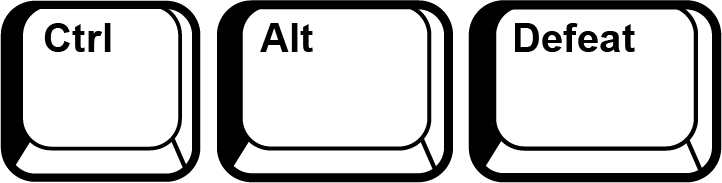
\includegraphics[width=6cm]{../../Images/cadLogo.png}

\end{titlepage}



\tableofcontents

\newpage

\section{Service Contract}

\subsection{Provided Software}
As per the agreement between the client and development team, the software "Domain Pulse: A Sentiment Analysis Platform" shall be developed and deployed within the given timeframe. The system will allow users to register, create domains, add sources for the domains, and view aggregated and analyzed sentiment data from the sources.

\subsection{Technology Stack}
The system will be developed using Django as the backend web framework and Angular for the frontend UI. MongoDB, a NoSQL database, will be used for sentiment data storage, while PostgreSQL will be employed for user data storage. The system will be deployed and hosted on a client-provided virtual machine.

\subsection{Project Management}
The project will be managed using the Agile methodology, with weekly meetings between team members for effective communication and task coordination. GitHub Project Boards will be used to track tasks and progress. Biweekly meetings with the client will be conducted to provide progress reports and sprint reviews.

\subsection{Module Agreement}
The developed system will consist of external services and libraries within the codebase, comprising no more than 15% of the total developed codebase. The team will ensure compliance with The University of Pretoria's Plagiarism and Code of Conduct policies, ensuring the originality and ownership of the produced code.

\subsection{Timeline}
The project will be completed within the provided timeframes of the COS 301 Capstone Project, and all required information and progress updates will be provided during the respective demos.

\subsection{Security}
Encryption will be implemented on all endpoints within the project to ensure secure data transmission between the server and the client. The virtual machine hosting the system will be secured and protected using measures such as firewalls. POST requests will be preferred over GET requests for enhanced data security.

\subsection{Law and User Privacy}
The software will comply with South African regulations, including laws such as the Protection of Personal Information Act (POPIA). User privacy and data will be protected and secured as required by the regulations.


\end{document}